\chapter{Implementación de los Algoritmos Propuestos}\label{cap4}


En este capítulo se describe el desarrollo de los algoritmos propuestos, cómo se implementaron y sobre qué tecnología. Se especifican los algoritmos a partir de pseudocódigos y se muestra cómo se interactúa con los mismos a partir del entorno de prueba implementado. Finalmente se muestra cómo se integraron los algoritmos desarrollados con el \emph{Algoritmo de Fuerzas de Tunkelang} y cómo se implementó sobre el entorno de prueba.

\section{Herramientas y Lenguajes Utilizados}
Para el desarrollo de la herramienta de prueba y depuración de los algoritmos se utilizó el IDE NetBeans y el lenguaje de programación Java. Se hicieron uso de las librerías Swing que provee Java para la creación de la interfaz gráfica que permite graficar Diagramas de Arcos e interactuar con ellos aplicándole los algoritmos de este trabajo, como también permite visualizar la integración con el algoritmo dirigido por fuerzas de Tunkelang, el cuál está implementado sobre la herramienta Jiggle (también desarrollada en Java).

\section{Aplicación de Algoritmos: Entorno de Prueba}
Los algoritmos presentados en las secciones \ref{sec:diseno_algoritmo_completo} y \ref{sec:diseno_algoritmo_arcgen}, tanto el que obtiene un óptimo Crossing Number para grafos completos, como su refinamiento para grafos no completos y finalmente, \textsc{ArcGen}, el algoritmo genético para mejorar el resultado, fueron implementados en lenguaje Java. % y testeados. %A continuación veremos algunos pseudocódigos de estos algoritmos, los cuales utilizan un
	La  representación de Diagrama de Arcos % que se utiliza es la explicada dada en la sección \ref{subsec:representacion_individuos}. 
	%como se mencionó, registra tres arreglos donde
	almacena los nodos, su orden y sus arcos. Los métodos que incluye son: intercambiar nodos, mover un nodo a una posición realizando intercambios, transponer arcos, calcular cruces del grafo y de un arco en particular, calcular grado de arcos y nodos, y nivel de nodo y clonar el grafo.
		\begin{figure}
	    \begin{center}
		\begin{algorithmic}[1]
			\REQUIRE Diagrama de Arcos.
			\STATE Ordenar los nodos según su nivel en orden descendiente.
			\STATE Determina si el número de nodos ($n$) es par o impar.
			\STATE Asigna a un $punteroIzquierdo$ la posición $n/2$.
			\IF {número de nodos par}
			\STATE $punteroDerecho$ comenzará en $n/2 - 1 $.
			\ELSE
			\STATE $punteroDerecho$ comenzará en $n/2 + 1 $.
			\ENDIF
			\STATE Determina el semiplano inicial donde graficar. Si $n$ es par superior sino inferior.
			\FORALL {nodo $\in$ Nodos del grafo}
			\IF {semiplano es superior}
			\STATE Graficar todos los arcos del nodo en $punteroIzquierdo$ en semiplano superior.
			\ELSE 
			\STATE Graficar todos los arcos del nodo en $punteroDerecho$ en semiplano inferior.
			\ENDIF
			\STATE Invierte el semiplano para la próxima iteración.
			\ENDFOR
			\STATE Llamar a algoritmo para optimizar grafo completo con el grafo trazado como entrada.
			\ENSURE Diagrama de Arcos optimizado.
		\end{algorithmic}
	    \end{center}

		\caption{Pseudocódigo para el trazado inicial de un Diagrama de Arcos.}
		\label{alg:arcdiagram_trazado}
	\end{figure}
    El algoritmo presentado en la Figura \ref{alg:arcdiagram_trazado}  realiza únicamente el trazado de los arcos como en la Figura \ref{fig:arcdiagram_k6_no_optimo}. Inicialmente,  ordena los nodos por su nivel. En  un grafo completo, el ordenamiento no produce ningún cambio, ya que todos sus nodos tienen el mismo nivel. Sin embargo, en los grafos no completos, permite un ordenamiento inicial más adecuado. Hay que considerar que el algoritmo realiza un recorrido desde el centro hacia los extremos a pesar de que la explicación inicial dada en la sección \ref{sec:diseno_algoritmo_completo} es a la inversa, esto es debido a la manera en que se da la implementación del Diagrama de Arcos y cómo se realizan los inversiones de arcos e intercambios de nodos internamente.
	Por último, el algoritmo invoca al algoritmo para optimizar grafos completos y elimina  los conflictos que genera.
	\begin{figure}
	    \begin{center}
		\begin{algorithmic}[1]
			\REQUIRE Diagrama de Arcos trazado.
			\STATE Calcula el número de transposiciones $t(n) = \floor*{\frac{n}{2}}-2$, con $n > 5$, sino $0$ en caso de $n \leq 5$.
			\STATE Asigna a un $punteroIzquierdo$ la posición 0.
			\STATE Asigna a un $punteroDerecho$ la posición $n-1$.
			\STATE Comienza apuntando al $punteroIzquierdo$.
			\FOR {$i = 0$ hasta $t(n)$}
			\STATE Obtiene los arcos del nodo en el puntero que apunte.
			\STATE Cambia el puntero al opuesto.
			\STATE Inicializa $intercambios$ en $t(n)-i$.
			\WHILE {$j < $ arcos del nodo \AND $intercambios > 0$}
			\STATE Calcula el $CrossingNumber$ actual.
			\STATE Obtiene la $distancia$ entre el nodo actual y el nodo al que conecta el arco.
			\IF {$1 < distancia \leq (t(n)-i+1)$}
			\STATE Invierte el semiplano del arco[$j$].
			\STATE Recalcula el $CrossingNumber$.
			\IF {$CrossingNumber$ es mayor al anterior}
			\STATE Invierte el semiplano del arco[$j$] nuevamente.
			\ENDIF
			\ENDIF
			\ENDWHILE
			\ENDFOR
			\ENSURE Diagrama de Arcos optimizado.
		\end{algorithmic}
	    \end{center}

		\caption{Pseudocódigo para la optimización de Diagrama de Arcos completos.}
		\label{alg:arcdiagram_optimizado}
	\end{figure}
	En el algoritmo descripto en la Figura \ref{alg:arcdiagram_optimizado} se presenta la optimización que soluciona los cruces conflictivos para grafos completos y permite obtener el Diagrama de Arcos inicial para lanzar el algoritmo genético.
	\begin{figure}	
	    \begin{center}
		\begin{algorithmic}[1]
			\REQUIRE Diagrama de Arcos optimizado para completo, un entero $maxCiclos$.
			\STATE Asigna una variable $igualCrossNum$ en falso.
			\WHILE {$i < maxCiclos$ \AND $igualCrossNum$ sea falso}
			\STATE Llamar a algoritmo de ciclo genético y obtener un nuevo grafo.
			\IF {$CrossingNumber$ del grafo anterior es igual al nuevo}
			\STATE Asigna a $igualCrossNum$ verdadero.
			\ENDIF
			\ENDWHILE
			\ENSURE Diagrama de Arcos con optimización genética.
		\end{algorithmic}
	    \end{center}

		\caption{Pseudocódigo para la optimización genética de Diagrama de Arcos no completos.}
		\label{alg:genetico}
	\end{figure}
	
	Finalmente,  se realiza la optimización con el algoritmo genético. El algoritmo presentado en la Figura \ref{alg:genetico} realiza las llamadas a cada ciclo de generaciones hasta encontrar dos ciclos con igual número de cruces o hasta cumplir con $100$ ciclos de tope. Cada ciclo es una llamada al algoritmo de 	generaciones [Figura \ref{alg:genetico_ciclo}], que genera poblaciones,  muta sus individuos, seleccionando los más aptos, esto es, aquellos  con menor número de cruces que el grafo semilla y devuelve el mejor grafo obtenido.
		

		
	
	%La generación de población inicial y procesos de mutación  son explicados en la sección \ref{sec:genetico}.
	
	
	%Para probar los algoritmos explicados en las secciones anteriores se ha desarrollado una aplicación [Fig. \ref{fig:aplicacion}] que permite la visualización de los Diagrama de Arcos y por otro lado  almacena los resultados de tiempo, ciclos, arcos generados, cruces iniciales y finales de la ejecución del algoritmo genético, siendo que las optimizaciones anteriores son computables rápidamente.
	

	

	\begin{figure}
	    \begin{center}
		\begin{algorithmic}[1]
			\REQUIRE Diagrama de Arcos de ciclo anterior, un entero $maxGeneraciones$.
			\STATE Calcula el $CrossingNumber$ del grafo de entrada, para comparar más adelante.
			\STATE Genera la población inicial con el grafo de entrada.
			\WHILE {$i < maxGeneraciones$ \AND grafo óptimo no encontrado}
			\FORALL {individuo de la población}
			\STATE Muta nodos del individuo con una probabilidad del 30\%.
			\STATE Muta arcos del individuo con una probabilidad del 10\%.
			\IF {individuo es un grafo óptimo (sin cruces)}
			\STATE Corta y devuelve el grafo óptimo.
			\ELSE
			\IF {individuo es peor que el original}
			\STATE Elimina al grafo de la población.
			\ENDIF
			\ENDIF
			\ENDFOR
			\IF {no se encontró grafo óptimo}
			\STATE Ordena los individuos por su fitness (menor CN).
			%\STATE Establece el mejor grafo obtenido de entre los individuos, considerando el mejor de las generaciones anteriores.
			\STATE Obtiene el primer individuo del conjunto (el de mejor fitness).
			% y verifica que tenga mejor fitness que el mejor obtenido en la generación anterior. Si es así lo establece como el mejor, caso contrario permanece el anterior.
			\IF {individuo tiene mejor fitness que mejor individuo de generaciones anteriores}
			\STATE Establece al nuevo individuo como el mejor obtenido.
			\ENDIF
			\ENDIF
			\ENDWHILE
			\ENSURE Diagrama de Arcos óptimo o mejor encontrado.
		\end{algorithmic}
	    \end{center}
		\caption{Pseudocódigo de un ciclo del algoritmo genético.}
		\label{alg:genetico_ciclo}
	\end{figure}
En la  Figura \ref{fig1:aplicacion}  se muestra la interfaz  de la aplicación desarrollada  que permite la visualización de los Diagramas de Arcos.
\begin{figure}
		\centering
		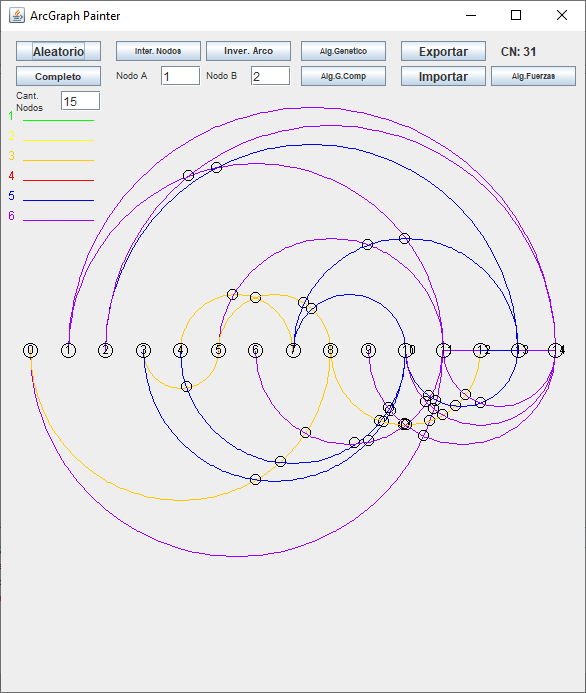
\includegraphics[scale=0.7]{imagenes/aplicacion.png}
		\caption{Interfaz de la aplicación desarrollada para visualizar resultados y experimentación.}
		\label{fig1:aplicacion}
	\end{figure}
	
	\begin{figure}
		\centering
		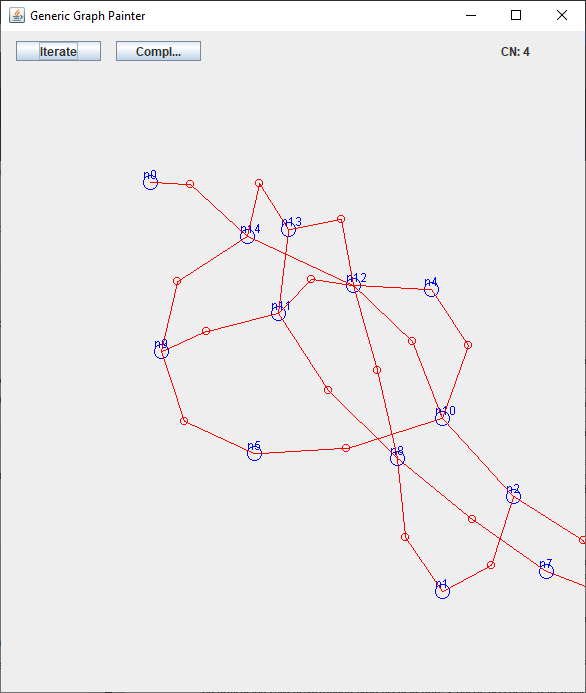
\includegraphics[scale=0.7]{imagenes/aplicacion_fuerzas.png}
		\caption{Ventana emergente de la aplicación para visualizar grafos luego de aplicar el algoritmo de Tunkelang.}
		\label{fig2:aplicacion}
	\end{figure}
Los números en los nodos representan su nombre o identificador,  y permiten diferenciar al nodo sin considerar el orden en que se disponen en la recta del Diagrama de Arcos.

Los arcos en el gráfico tienen diferentes colores de acuerdo a su {\em grado de arco}, a fin   de visualizar aquellos nodos con más relaciones, según los arcos que conecta. Los colores de arcos verde, amarillo, naranja, rojo, azul y violeta identifican el grado de arco 1, 2, 3, 4, 5 y 6 respectivamente. Todo aquel arco con grado mayor a 6 es representado con color negro.

En la esquina superior derecha se encuentra un campo de texto etiquetado como \texttt{CN} que muestra el crossing number sobre el grafo que se está mostrando actualmente.


También se dispone de una serie de botones que brindan varias funcionalidades. Los botones \texttt{Aleatorio} y \texttt{Completo} permiten generar grafos aleatorio o completos, respectivamente, dada la cantidad de nodos que se especifican en la ventana de texto de texto etiquetada como \texttt{Cant. Nodos}. 

Los botones \texttt{Inter. Nodos} y \texttt{Inver. Arco} en la  Figura \ref{fig1:aplicacion}\ permiten invertir el orden de los nodos y transponer un arco dado entre dos nodos, respectivamente, obteniendo los identificadores de los nodos desde las ventanas de texto etiquetadas como \texttt{Nodo A} y \texttt{Nodo B}. 

Los botones \texttt{Alg. Genético} y \texttt{Alg. G. Comp} permiten lanzar el algoritmo genético \textsc{ArcGen} o el algoritmo para grafos completos respectivamente, sobre el grafo que se está visualizando actualmente, y luego lo reemplaza por el resultado. Asimismo,  almacena los resultados de tiempo, ciclos, arcos generados, cruces iniciales y finales de la ejecución del algoritmo.

El botón \texttt{Alg. Fuerzas} permite ejecutar el algoritmo de fuerzas de Tunkelang sobre el grafo actualmente visualizado, luego  de realizarle al Diagrama de Arcos la transformación a grafo genérico que se explica en la sección \ref{sec:integracion_tunkelang}. Una nueva ventana  muestra la gráfica del resultado, indicando su crossing number, como se ve en la Figura   \ref{fig2:aplicacion}.

Los botones \texttt{Exportar} e \texttt{Importar} en la Figura \ref{fig1:aplicacion}\ permiten exportar e importar respectivamente, Diagramas de Arcos, utilizando un formato XML con una estructura propia de la aplicación. En la Figura \ref{fig:ejemplo_xml} se muestra un ejemplo de un Diagrama de Arcos exportado en el formato XML. El archivo XML contiene la información de todos los  nodos del grafo y su orden en el dibujo y de  todos los arcos y el semiplano en el que están dibujados  (1: semiplano  superior; 0: semiplano inferior).

\begin{figure}

	\centering
	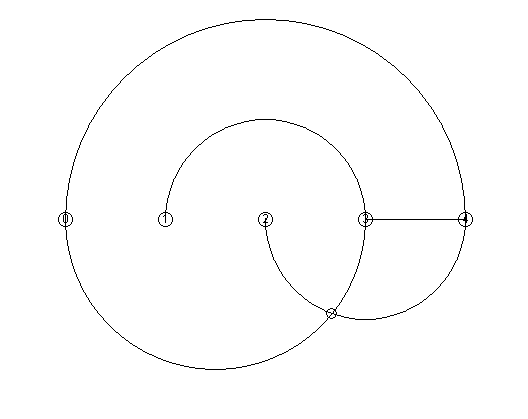
\includegraphics[width=15cm]{imagenes/ejemplo_xml.png}
	\begin{multicols}{2}
\begin{minted}[obeytabs=true,tabsize=2]{xml}
<?xml version="1.0" encoding="UTF-8"?>
<diagram>
  <nodes>
    <node order="0">0</node>
    <node order="1">1</node>
    <node order="2">2</node>
    <node order="3">3</node>
    <node order="4">4</node>
  </nodes>
  <edges>
    <edge direction="1">
      <node>0</node>
      <node>4</node>
    </edge>
    <edge direction="0">
      <node>0</node>
      <node>3</node>
    </edge>
    <edge direction="1">
      <node>1</node>
      <node>3</node>
    </edge>
    <edge direction="0">
      <node>2</node>
      <node>4</node>
    </edge>
    <edge direction="1">
      <node>3</node>
      <node>4</node>
    </edge>
  </edges>
</diagram>
\end{minted}
\end{multicols}
	\caption{Ejemplo de grafo exportado en formato XML por la herramienta.}
	\label{fig:ejemplo_xml}
\end{figure}



%En la parte inferior encontramos los valores \texttt{Population}, \texttt{E.Time} y \texttt{E.Cycles} que indican el tamaño de la población, el tiempo y la cantidad de ciclos, estimados según los registros guardados para el algoritmo genético.	
%\todo[inline]{almacena o  solo muestra???}

%\todo[inline,color=softred]{R: los almacena, cada vez que se ejecuta el genetico guarda los datos de tiempo, ciclos, etc, y actualiza los valores que muestra en la aplicacion (que son promedios de los guardados).}
%, siendo que las optimizaciones anteriores son computables rápidamente.
\ \\
\ \\
La aplicación está  desarrollada bajo licencia libre y puede accederse a la versión más reciente de su ejecutable a través del repositorio de BitBucket:\\  \url{https://bitbucket.org/giuliano-marinelli/graphlayout}

\section{Integración con el Algoritmo Dirigido por Fuerzas de Tunkelang}
\label{sec:integracion_tunkelang}
El resultado obtenido por los algoritmos de este trabajo no disponen una visualización genérica amigable para el usuario, ya que se centran en la resolución de crossing number sobre grafos con estilo de dibujado de Diagrama de Arcos, como se explica en la sección \ref{sec:integracion_generico}. Para poder lograr una aproximación a un resultado práctico se utiliza el algoritmo de fuerzas de Tunkelang \cite{tunkelang1998jiggle} sobre los grafos resultantes, aunque podrían utilizarse otros algoritmos, como el algoritmo de  ortogonal. 

Brevemente, el algoritmo de Tunkelang se basa en aplicar fuerzas de atracción y repulsión entre los nodos del grafo durante un tiempo determinado, de manera que éstos se reacomoden en el plano y se obtenga un disposición más distribuida de los mismos. En el capítulo \ref{cap_trabajos_relacionados} se explican más detalles del algoritmo. Para lectores interesados en  una descripción más particularizada ver Tunkelang et al. \cite{tunkelang1998jiggle}.

El algoritmo de fuerzas no puede aplicarse de forma directa sobre el Diagrama de Arcos, ya que es una estructura de datos distinta a la que utiliza el algoritmo. Es necesario aplicar una transformación en la representación para lograr que éste disponga de la estructura de datos necesaria. En este sentido, se transforma la representación que se planteó en la sección \ref{subsec:representacion_individuos} en un nuevo objeto, donde se registra cada nodo con su posición $(x,y)$ en el plano y cada vértice como una línea recta que une cada nodo. En consecuencia, a partir del Diagrama de Arcos se generaría un grafo donde todos los arcos estarían dibujados de manera superpuesta con la línea en la que se encuentran los nodos.%, ya que los arcos en el Diagrama de Arcos están dibujados como líneas curvas.

Para lograr que los arcos puedan transformarse en líneas rectas sin perder la forma del grafo se crearon nuevos nodos, diferenciados de los nodos originales, llamados ``nodos de inflexión", los cuales se colocan en alguna parte del trayecto de la línea curva que se dibuja para cada arco y conectan con los nodos originales, a partir de dos arcos que reemplazarán al arco original, como se muestra en la Figura \ref{fig:transformacion_arc_generico}. Luego a partir de este grafo resultante, representado como un objeto con sus posiciones en el plano es posible aplicar el algoritmo de fuerzas para obtener el resultado final.

\begin{figure}
	\centering
	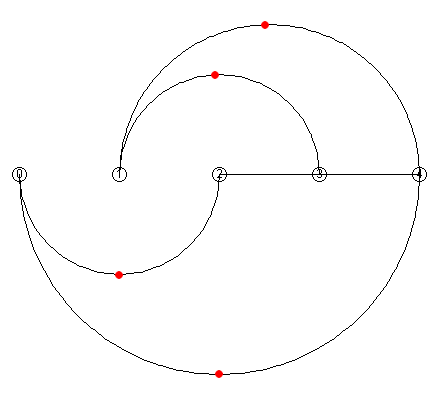
\includegraphics[width=8cm]{imagenes/transformacion_arc_generico_1.png}
	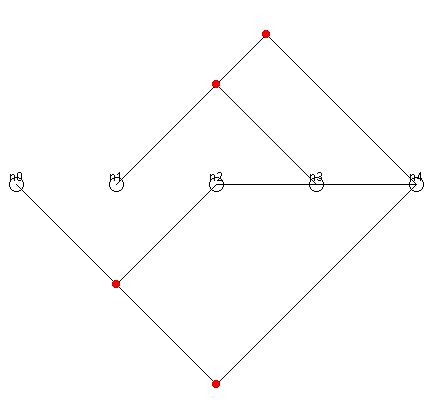
\includegraphics[width=8cm]{imagenes/transformacion_arc_generico_3.png}
	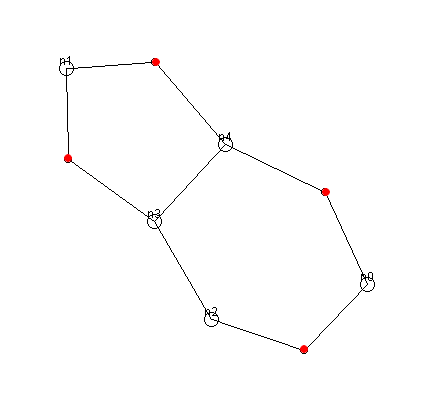
\includegraphics[width=8cm]{imagenes/transformacion_arc_generico_2.png}
	\caption{Transformación de un diagrama de arcos a un grafo genérico, utilizando nodos de inflexión (marcados en rojo), y resultado final aplicando algoritmo de fuerzas de Tunkelang.}
	\label{fig:transformacion_arc_generico}
\end{figure}